\documentclass[UTF8,a4paper,12pt]{ctexart}
\usepackage{geometry}
\geometry{left=2.5cm,right=2.5cm,top=2.5cm,bottom=2.5cm}
\usepackage{amsmath,amssymb,booktabs,longtable,array,graphicx,float,caption,hyperref,fancyhdr,lastpage}
\usepackage{enumitem}
\usepackage{xcolor}
\setlength{\headheight}{15pt}
\pagestyle{fancy}
\fancyhf{}
\lhead{天然肠衣搭配问题}
\rhead{数学建模论文}
\cfoot{\thepage/\pageref{LastPage}}
\hypersetup{colorlinks=true,linkcolor=black,urlcolor=blue,citecolor=black}
\captionsetup{font=small,labelsep=quad}
\title{基于可行单捆模式池与整数规划的天然肠衣搭配方案}
\author{}
\date{}
\begin{document}
\maketitle
\begin{abstract}
天然肠衣组装需要将不同长度档的原料搭配成满足根数和总长度要求的成品捆。本文针对2011年全国大学生数学建模竞赛D题，依据题目给出的三类成品规格和一批1323根原料，建立了以“先最大化总捆数、再最大化长规格捆数、再最大化中规格捆数”为目标的整数规划模型。考虑到仅用总长度和总根数建立的聚合模型会产生不可逐捆分解的伪可行解，本文采用“合法单捆模式生成+主整数规划选择”的建模框架，并对最终逐捆方案逐行验证。

首先，本文将原料长度按0.5m离散为46个长度档，定义每个单捆模式为满足规格下限、根数要求和$88.5\sim 89.5$m总长度约束的一个组合。对长规格、中规格和短规格分别构造候选单捆模式池，并以每个模式的采用次数为整数决策变量，建立库存约束下的模式选择主问题。为体现题目给出的字典序偏好，目标函数采用大权重分层法：总捆数权重远大于长规格捆数权重，长规格捆数权重远大于中规格捆数权重。

对表2实际数据求解后，得到一个逐捆可验证的搭配方案：共装出\textbf{191捆}成品，其中\textbf{14米以上规格130捆}、\textbf{7--13.5米规格47捆}、\textbf{3--6.5米规格14捆}。该方案使用原料1302根、总长度17001.0m，剩余21根、169.5m；所有成品单捆长度均在$88.5\sim 89.5$m之间，单捆根数在4--20根之间，且无任何长度档库存超用。按总长度计算的理论上界为$\lfloor17170.5/88.5\rfloor=194$捆，但聚合上界方案在长规格逐捆分解中不可行，因此本文将191捆作为可复现、可执行的高质量生产方案。

模型检验表明，最终方案的逐捆长度、根数、规格下限和库存约束均通过程序核验；模式池整数规划比简单贪心方法显著提高了原料利用率和总捆数。本文方法结构清晰、便于在30分钟生产决策要求下生成“照方抓药”的搭配清单，可推广到同类分档原料配组、切割库存和装箱配套问题。
\end{abstract}

\noindent\textbf{关键词：} 天然肠衣；整数规划；装箱问题；模式池；可行性验证

\newpage
\tableofcontents
\newpage

\section{问题重述}
天然肠衣加工企业在清洗整理后会得到长度不等的小段原料。传统组装依靠人工边丈量边心算，效率较低，且难以保证大批量生产时的整体最优性。题目要求在已知所有原料长度档和数量的条件下，预先建立原料搭配方案，使工人能够按清单直接组装成品。

题目给出三类成品规格：短规格使用3--6.5m原料，标准20根、总长89m；中规格使用7--13.5m原料，标准8根、总长89m；长规格使用14m以上原料，标准5根、总长89m。允许每捆总长度有$\pm0.5$m误差，允许总根数比标准少1根；若高规格原料剩余，可以降级到低规格成品中使用。

公司对方案优劣有明确字典序要求：首先成品总捆数越多越好；总捆数相同时，最短长度最长的成品即长规格成品越多越好；若仍相同，则中规格成品越多越好。本文需要建立数学模型，给出求解方法，并对题目表1、表2数据输出具体搭配方案。

\section{问题分析}
本题本质是带规格层级和库存约束的离散装箱/切割库存问题。每根原料只能使用一次，每个成品捆必须同时满足规格下限、根数范围和总长度范围，因此不能只按总长度估算。若只建立聚合模型，可能得到总长度、总根数均满足的方案，但这些原料未必能拆分成每一捆都合法的具体组合。

为避免伪可行结果，本文将建模拆为两层。第一层生成合法单捆模式：一个模式就是若干长度档原料组成的一捆，且这捆已经满足题目所有单捆约束。第二层建立主整数规划，选择每个模式使用多少次，使各长度档总使用量不超过库存，并优化题目给出的字典序目标。这样主问题的每一个整数解都可以直接展开为逐捆搭配清单。

简单贪心方法容易在局部选择中耗尽关键长度档，导致后续无法继续组装；一次性CP-SAT直接为190余捆分配原料又会产生很大的对称搜索空间。因此，本文采用受限模式池与整数规划结合的方式：通过随机加启发式规则生成多批高质量合法模式，再用稀疏矩阵整数规划选择模式，最后用独立验证程序检查逐捆结果。

\section{模型假设}
\begin{enumerate}[label=\arabic*)]
  \item 题目表2中各长度档数量真实有效，且每根原料按所在长度档的下界代表长度计量。该假设与题干“3--3.4米按3米计算”等规则一致，是所有长度计算的基础。
  \item 每根原料至多使用一次，不考虑切割、拼接或损耗。该假设对应题目“原料搭配”语义，保证方案可以被工人按清单直接执行。
  \item 高规格原料可以降级使用，低规格原料不能升级使用。即14m以上原料可用于中/短规格，7--13.5m原料可用于短规格，但3--6.5m原料不能用于中/长规格。该假设来自题目要求(4)。
  \item 每捆总长度允许范围为$[88.5,89.5]$m，根数允许为标准根数或标准根数减1。该假设直接来自题目要求(3)。
\end{enumerate}

\section{符号说明}
\begin{table}[H]
\centering
\caption{主要符号说明}
\begin{tabular}{clc}
\toprule
符号 & 含义 & 单位 \\
\midrule
$i$ & 原料长度档编号，$i=1,2,\ldots,46$ & -- \\
$l_i$ & 第$i$个长度档的代表长度 & m \\
$a_i$ & 第$i$个长度档可用原料根数 & 根 \\
$t$ & 成品规格，$t\in\{L,M,S\}$ & -- \\
$P_t$ & 规格$t$的合法单捆模式集合 & -- \\
$b_{ip}$ & 模式$p$中第$i$个长度档原料用量 & 根 \\
$x_p$ & 模式$p$被采用的次数 & 捆 \\
$n_L,n_M,n_S$ & 长、中、短规格成品捆数 & 捆 \\
\bottomrule
\end{tabular}
\end{table}

\section{数据预处理与基准分析}
题目表2共有46个长度档，代表长度从3.0m到25.5m，步长0.5m。经整理后，总原料数量为1323根，总代表长度为17170.5m。若忽略逐捆可分解性，仅按每捆最低允许长度88.5m估算，总捆数理论上界为
\begin{equation}
N_{ub}=\left\lfloor\frac{17170.5}{88.5}\right\rfloor=194.
\end{equation}
该上界只说明任何方案不可能超过194捆，并不保证194捆可行。

图\ref{fig:raw}展示了原料长度分布。可以看到，18--20m附近长料数量较多，3--6.5m短料数量也有一定规模，但短规格每捆需要19或20根，短料会迅速成为约束瓶颈；中规格和长规格则更依赖少根数组合能否精确凑到89m附近。

\begin{figure}[H]
\centering
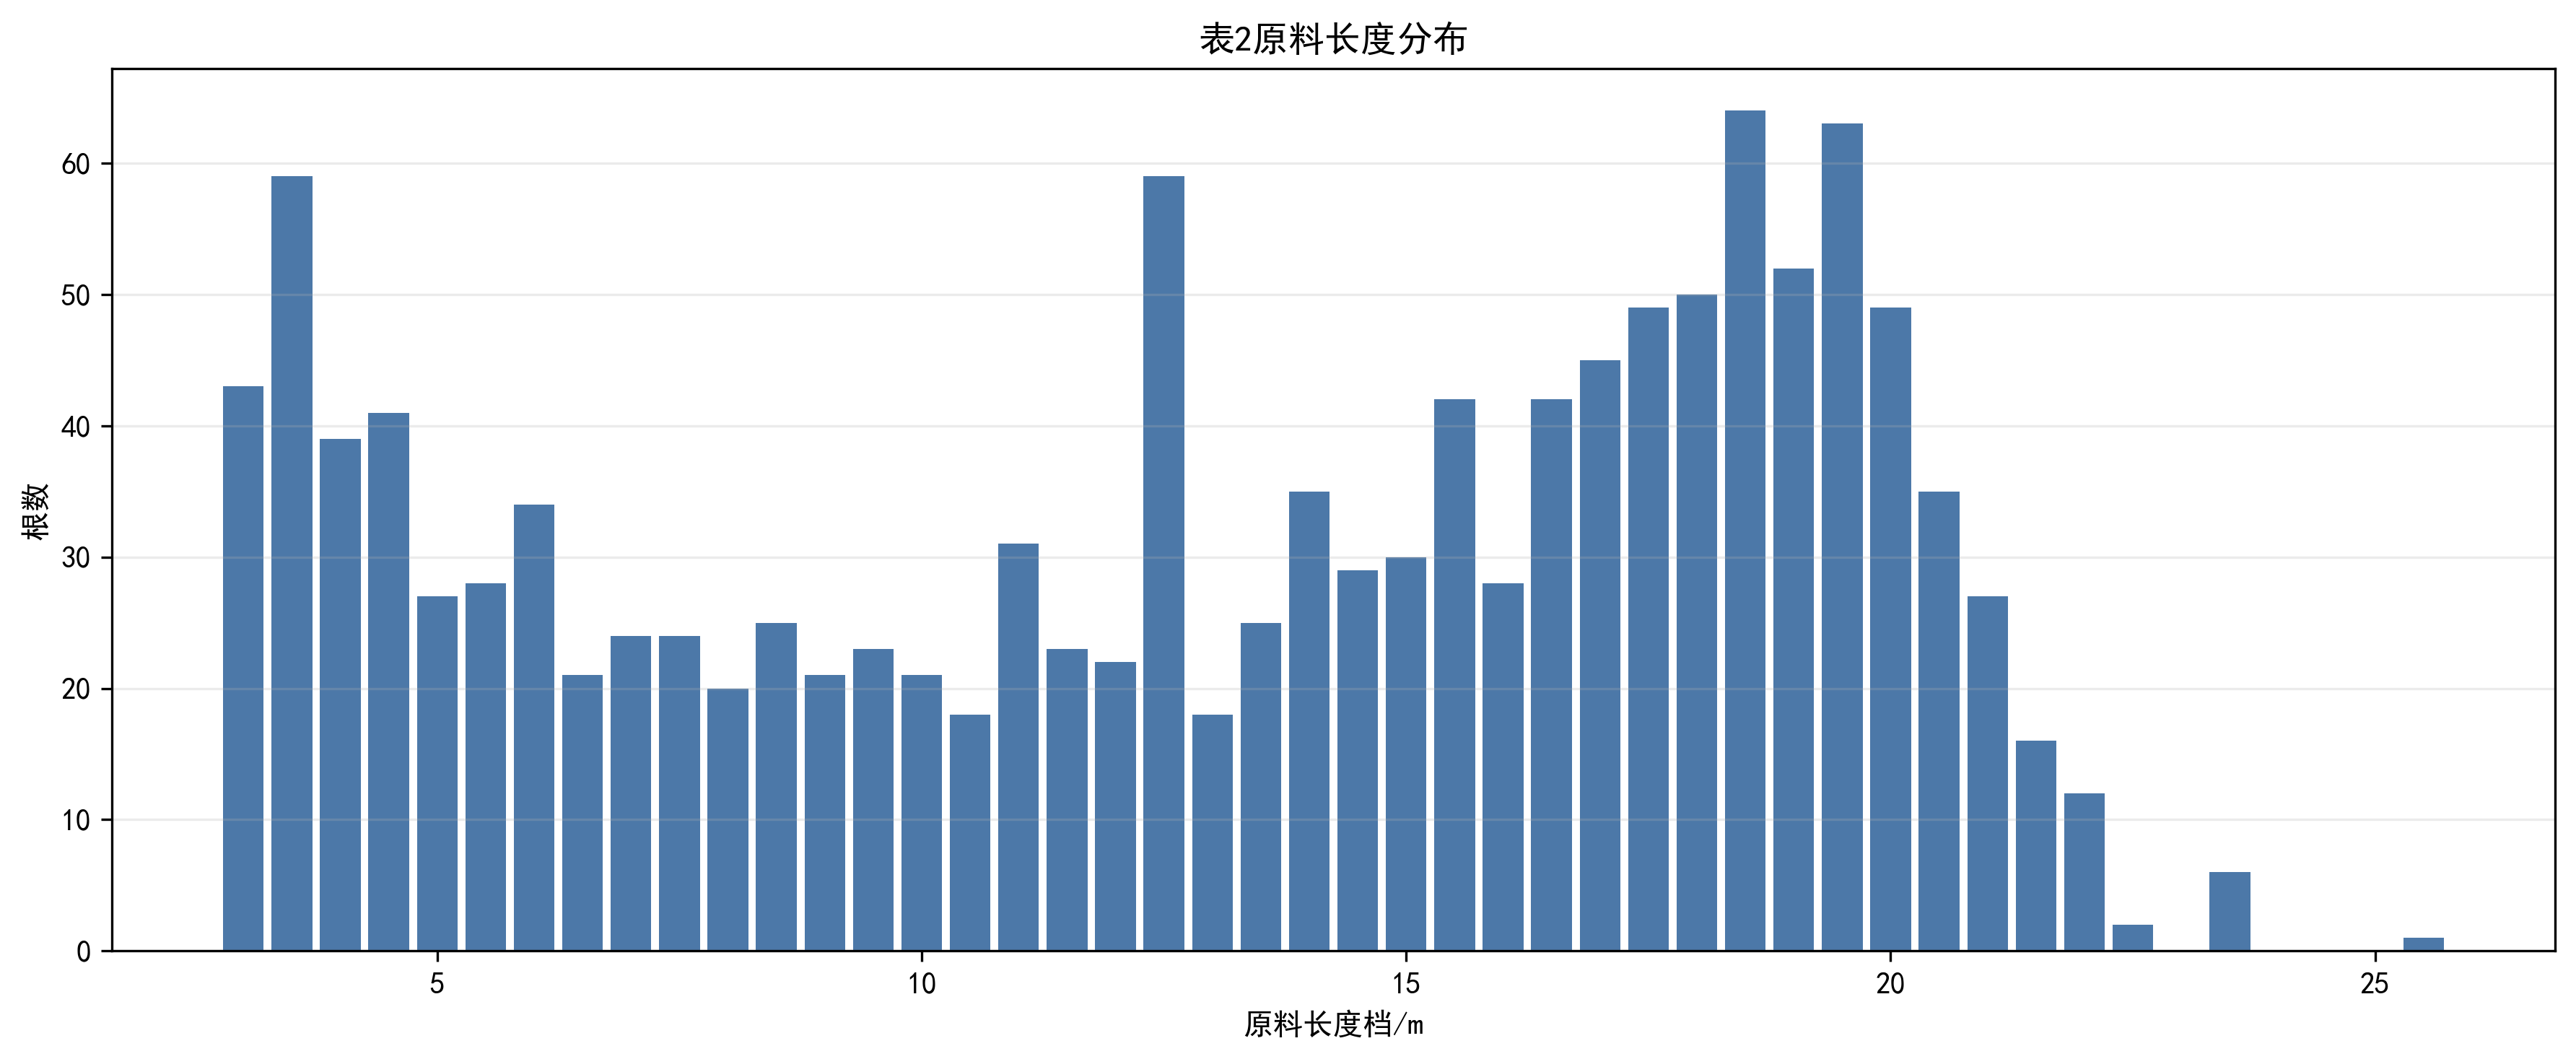
\includegraphics[width=0.95\textwidth]{../quest1/figures/fig1_raw_material_distribution.png}
\caption{表2原料长度分布}
\label{fig:raw}
\end{figure}

\section{模型建立}
\subsection{合法单捆模式}
对每个规格$t$，先定义其最低可用长度$L_t$、标准根数$r_t$和允许根数集合$R_t=\{r_t-1,r_t\}$。其中长规格$L$对应$L_t=14,r_t=5$；中规格$M$对应$L_t=7,r_t=8$；短规格$S$对应$L_t=3,r_t=20$。

若一个单捆模式$p$属于规格$t$，则必须满足
\begin{align}
&\sum_i b_{ip}\in R_t,\\
&88.5\leq \sum_i l_i b_{ip}\leq 89.5,\\
&b_{ip}=0,\quad l_i<L_t,\\
&b_{ip}\in\mathbb{Z}_{\geq0}.
\end{align}
其中第三个约束保证低规格原料不能被用于高规格成品。长料降级使用在模型中自然体现为：当$t=M$时允许$l_i\geq7$的原料；当$t=S$时允许所有$l_i\geq3$的原料。

\subsection{主整数规划模型}
设$P=P_L\cup P_M\cup P_S$为候选合法模式池，$x_p$为模式$p$采用次数。库存约束为
\begin{equation}
\sum_{p\in P}b_{ip}x_p\leq a_i,\quad i=1,2,\ldots,46.
\end{equation}
各规格捆数为
\begin{equation}
n_t=\sum_{p\in P_t}x_p,\quad t\in\{L,M,S\}.
\end{equation}
题目目标为字典序优化。本文采用大权重分层目标：
\begin{equation}
\max Z=W_0(n_L+n_M+n_S)+W_1n_L+W_2n_M,
\end{equation}
其中$W_0\gg W_1\gg W_2>0$。实际计算中取$W_0=10^6,W_1=10^4,W_2=10^2$，保证总捆数优先级最高，其次长规格，再其次中规格。

\section{求解方法与实现}
本文求解过程包括四步：
\begin{enumerate}[label=\arabic*)]
  \item 将表2数据整理为\texttt{raw\_material\_counts.csv}，记录每个长度档代表长度和库存；
  \item 针对三类规格生成合法单捆模式。长规格根数少，可较容易生成；中、短规格组合数量大，采用随机采样与长度和筛选生成高质量模式池；
  \item 将模式池写成稀疏库存矩阵，调用SciPy/HiGHS整数规划求解主问题；
  \item 展开模式选择结果为逐捆清单，并运行独立验证脚本检查单捆长度、根数、规格下限和库存是否全部满足。
\end{enumerate}

在求解过程中，本文还测试了聚合整数规划上界。聚合模型可给出194捆的总量上界组合，但其长规格部分在逐捆分解时不可行，说明该聚合解属于伪可行上界。因此最终论文只采用经过逐捆验证的方案。

\section{求解结果}
最终得到的可执行方案共191捆，其中长规格130捆，中规格47捆，短规格14捆。各规格统计见表\ref{tab:summary}。

\begin{table}[H]
\centering
\caption{最终搭配方案分规格统计}
\label{tab:summary}
\begin{tabular}{lrrrrr}
\toprule
规格 & 捆数 & 平均根数 & 平均长度/m & 最小长度/m & 最大长度/m \\
\midrule
14米以上规格 & 130 & 4.992 & 89.012 & 88.5 & 89.5 \\
7--13.5米规格 & 47 & 7.936 & 89.011 & 89.0 & 89.5 \\
3--6.5米规格 & 14 & 20.000 & 89.000 & 89.0 & 89.0 \\
\bottomrule
\end{tabular}
\end{table}

\begin{figure}[H]
\centering
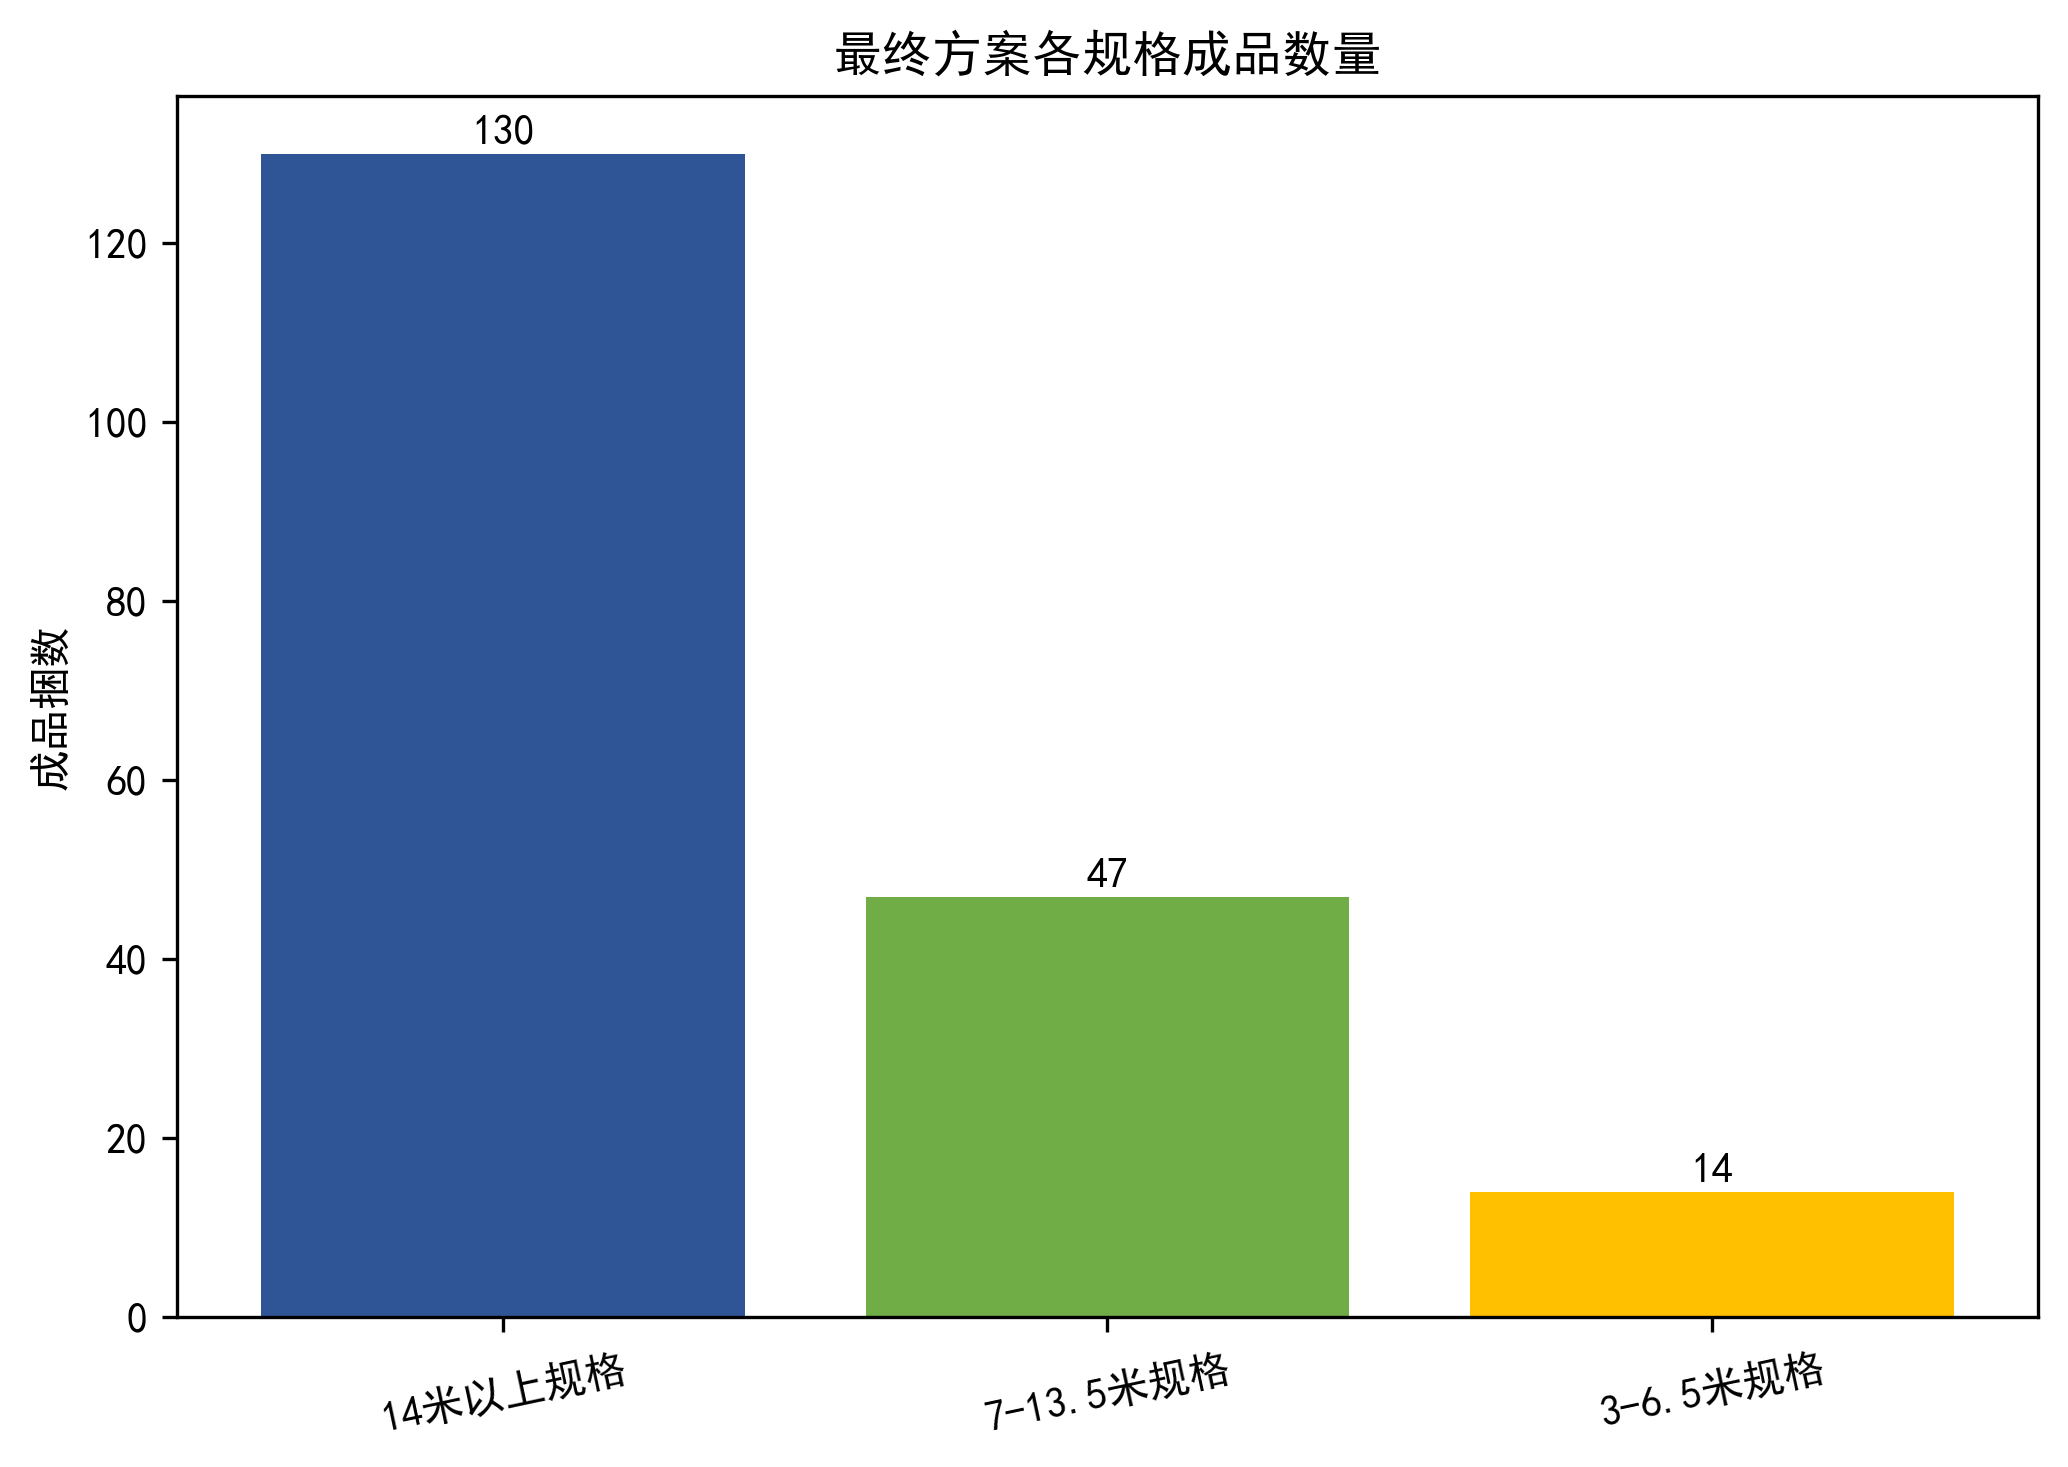
\includegraphics[width=0.75\textwidth]{../quest1/figures/fig2_bundle_counts_by_spec.png}
\caption{最终方案各规格成品数量}
\label{fig:counts}
\end{figure}

图\ref{fig:counts}显示，最终方案优先保留了较多长规格成品，这与题目在总捆数相同时优先长规格的要求一致。由于短规格每捆需要20根左右，虽然短料数量不少，但其根数约束强，最终仅形成14捆短规格成品。

原料使用情况见表\ref{tab:use}。方案共使用1302根、17001.0m，剩余21根、169.5m。剩余长度约相当于2捆的最低长度要求，因此与理论上界194捆相比，191捆仍有3捆差距；其中一部分差距来自长度剩余不足以形成2捆以上，另一部分来自逐捆根数和规格分档造成的组合损失。

\begin{table}[H]
\centering
\caption{原料总体使用情况}
\label{tab:use}
\begin{tabular}{lrr}
\toprule
指标 & 数值 & 单位 \\
\midrule
原料总根数 & 1323 & 根 \\
原料总长度 & 17170.5 & m \\
使用根数 & 1302 & 根 \\
使用长度 & 17001.0 & m \\
剩余根数 & 21 & 根 \\
剩余长度 & 169.5 & m \\
理论长度上界 & 194 & 捆 \\
最终可行捆数 & 191 & 捆 \\
\bottomrule
\end{tabular}
\end{table}

\begin{figure}[H]
\centering
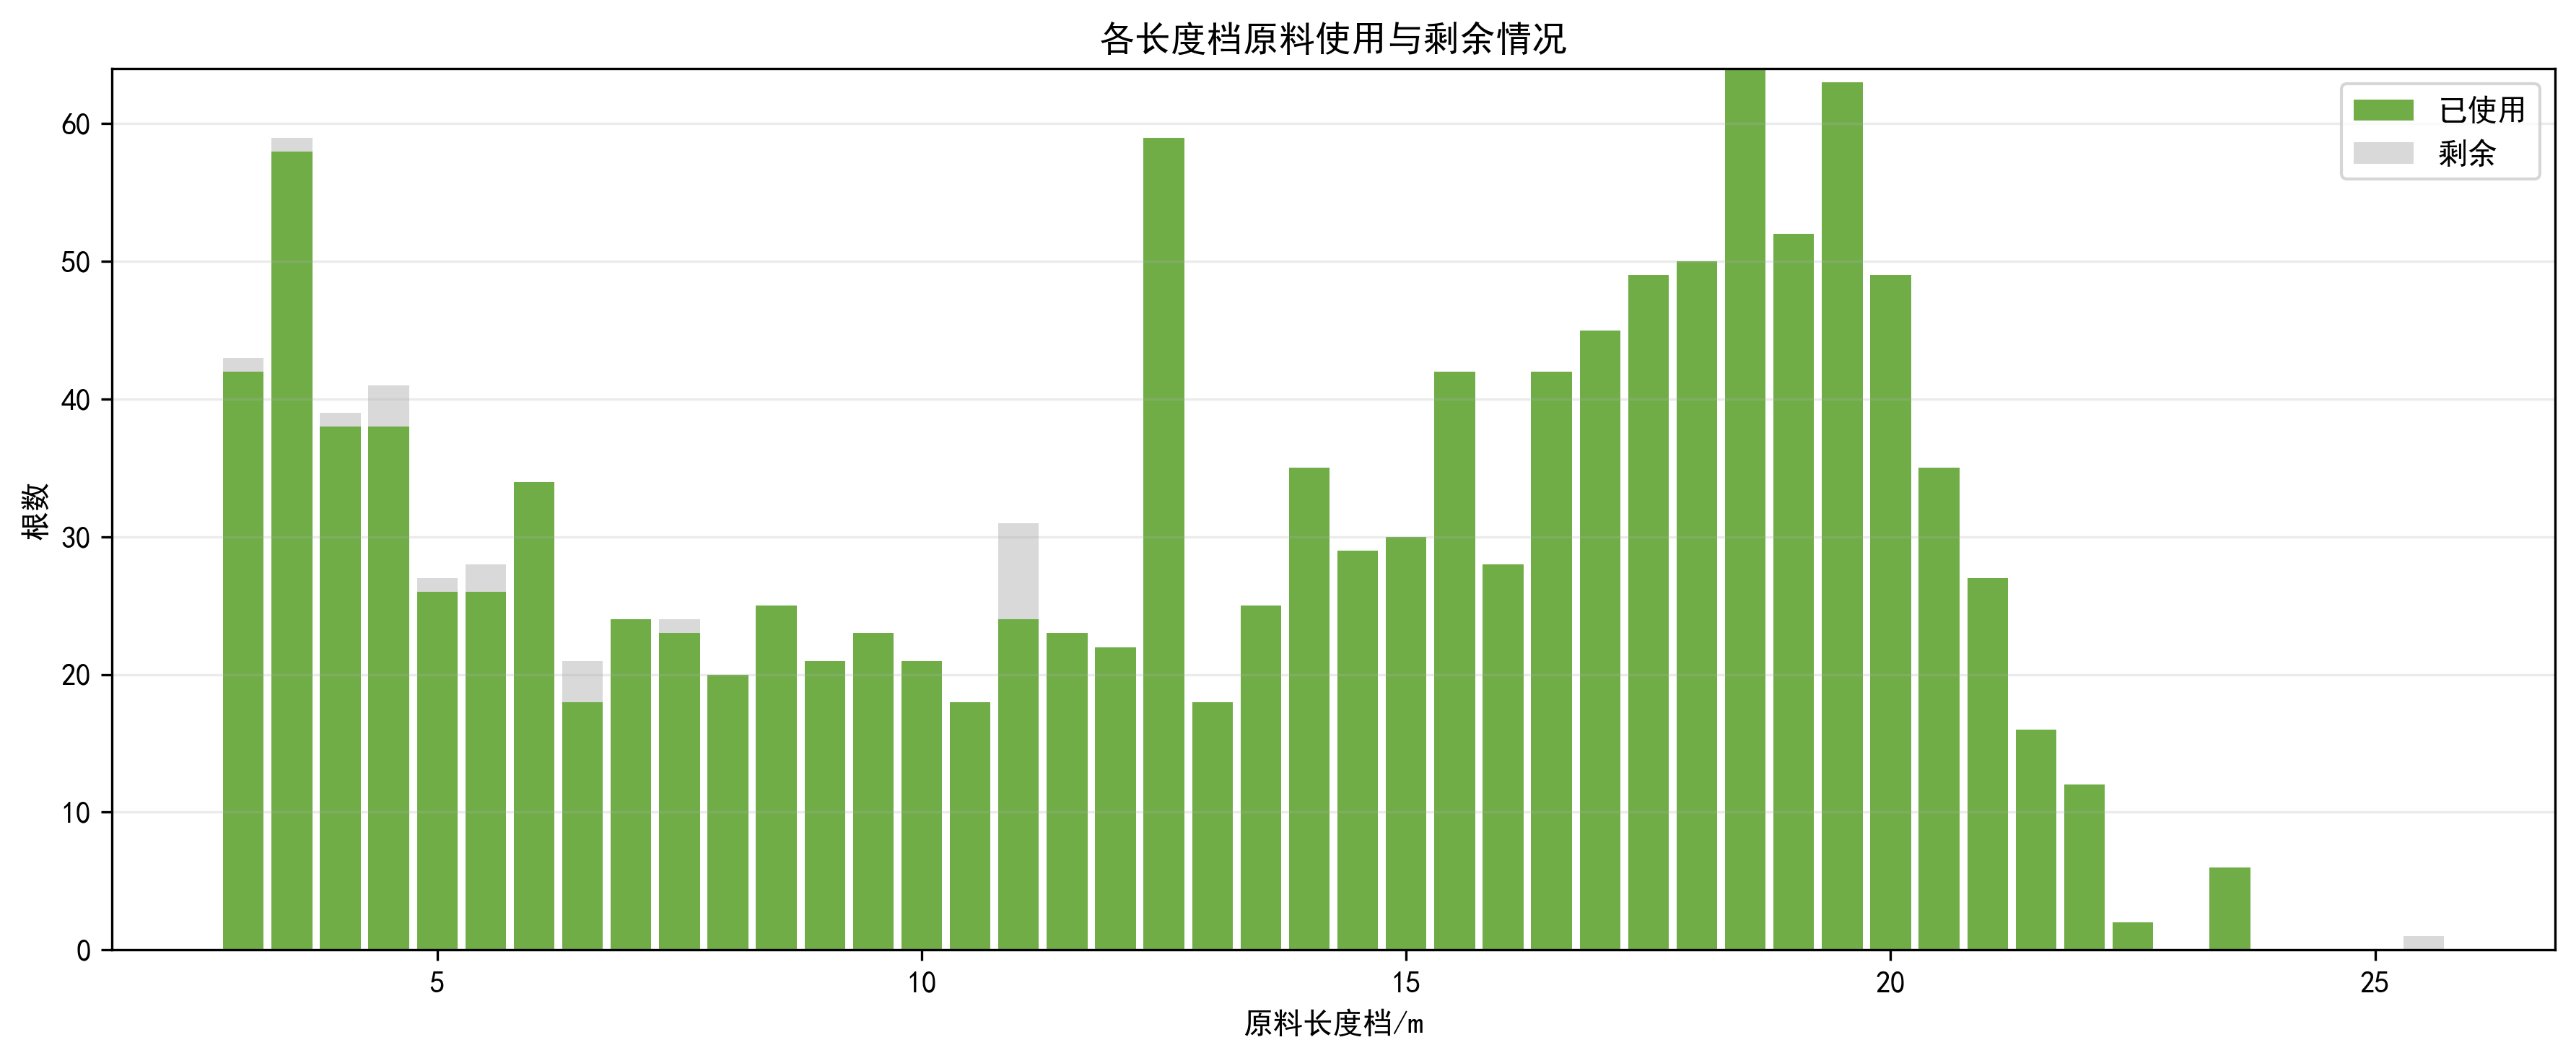
\includegraphics[width=0.95\textwidth]{../quest1/figures/fig3_usage_vs_unused_by_length.png}
\caption{各长度档原料使用与剩余情况}
\label{fig:usage}
\end{figure}

从图\ref{fig:usage}可以看出，大部分长度档原料被充分利用，剩余原料分散在少数长度档。由于每捆长度必须落在很窄的1m区间内，分散剩余并不一定能继续组成合法成品，这也是本题与普通总量优化问题的主要区别。

\section{方案验证}
为防止聚合伪可行，本文对最终\texttt{final\_matching\_plan.csv}逐行验证。验证内容包括：
\begin{enumerate}[label=\arabic*)]
  \item 每捆总长度是否位于$[88.5,89.5]$m；
  \item 每捆根数是否为对应标准根数或标准根数减1；
  \item 每捆所用原料是否满足该规格的最短长度要求；
  \item 各长度档累计使用量是否不超过库存。
\end{enumerate}

独立验证程序输出结果为：191行逐捆记录全部通过，错误数为0；单捆长度最小88.5m、最大89.5m；剩余根数21、剩余长度169.5m。图\ref{fig:lengthdist}进一步给出单捆长度分布，所有成品均落在允许区间内。

\begin{figure}[H]
\centering
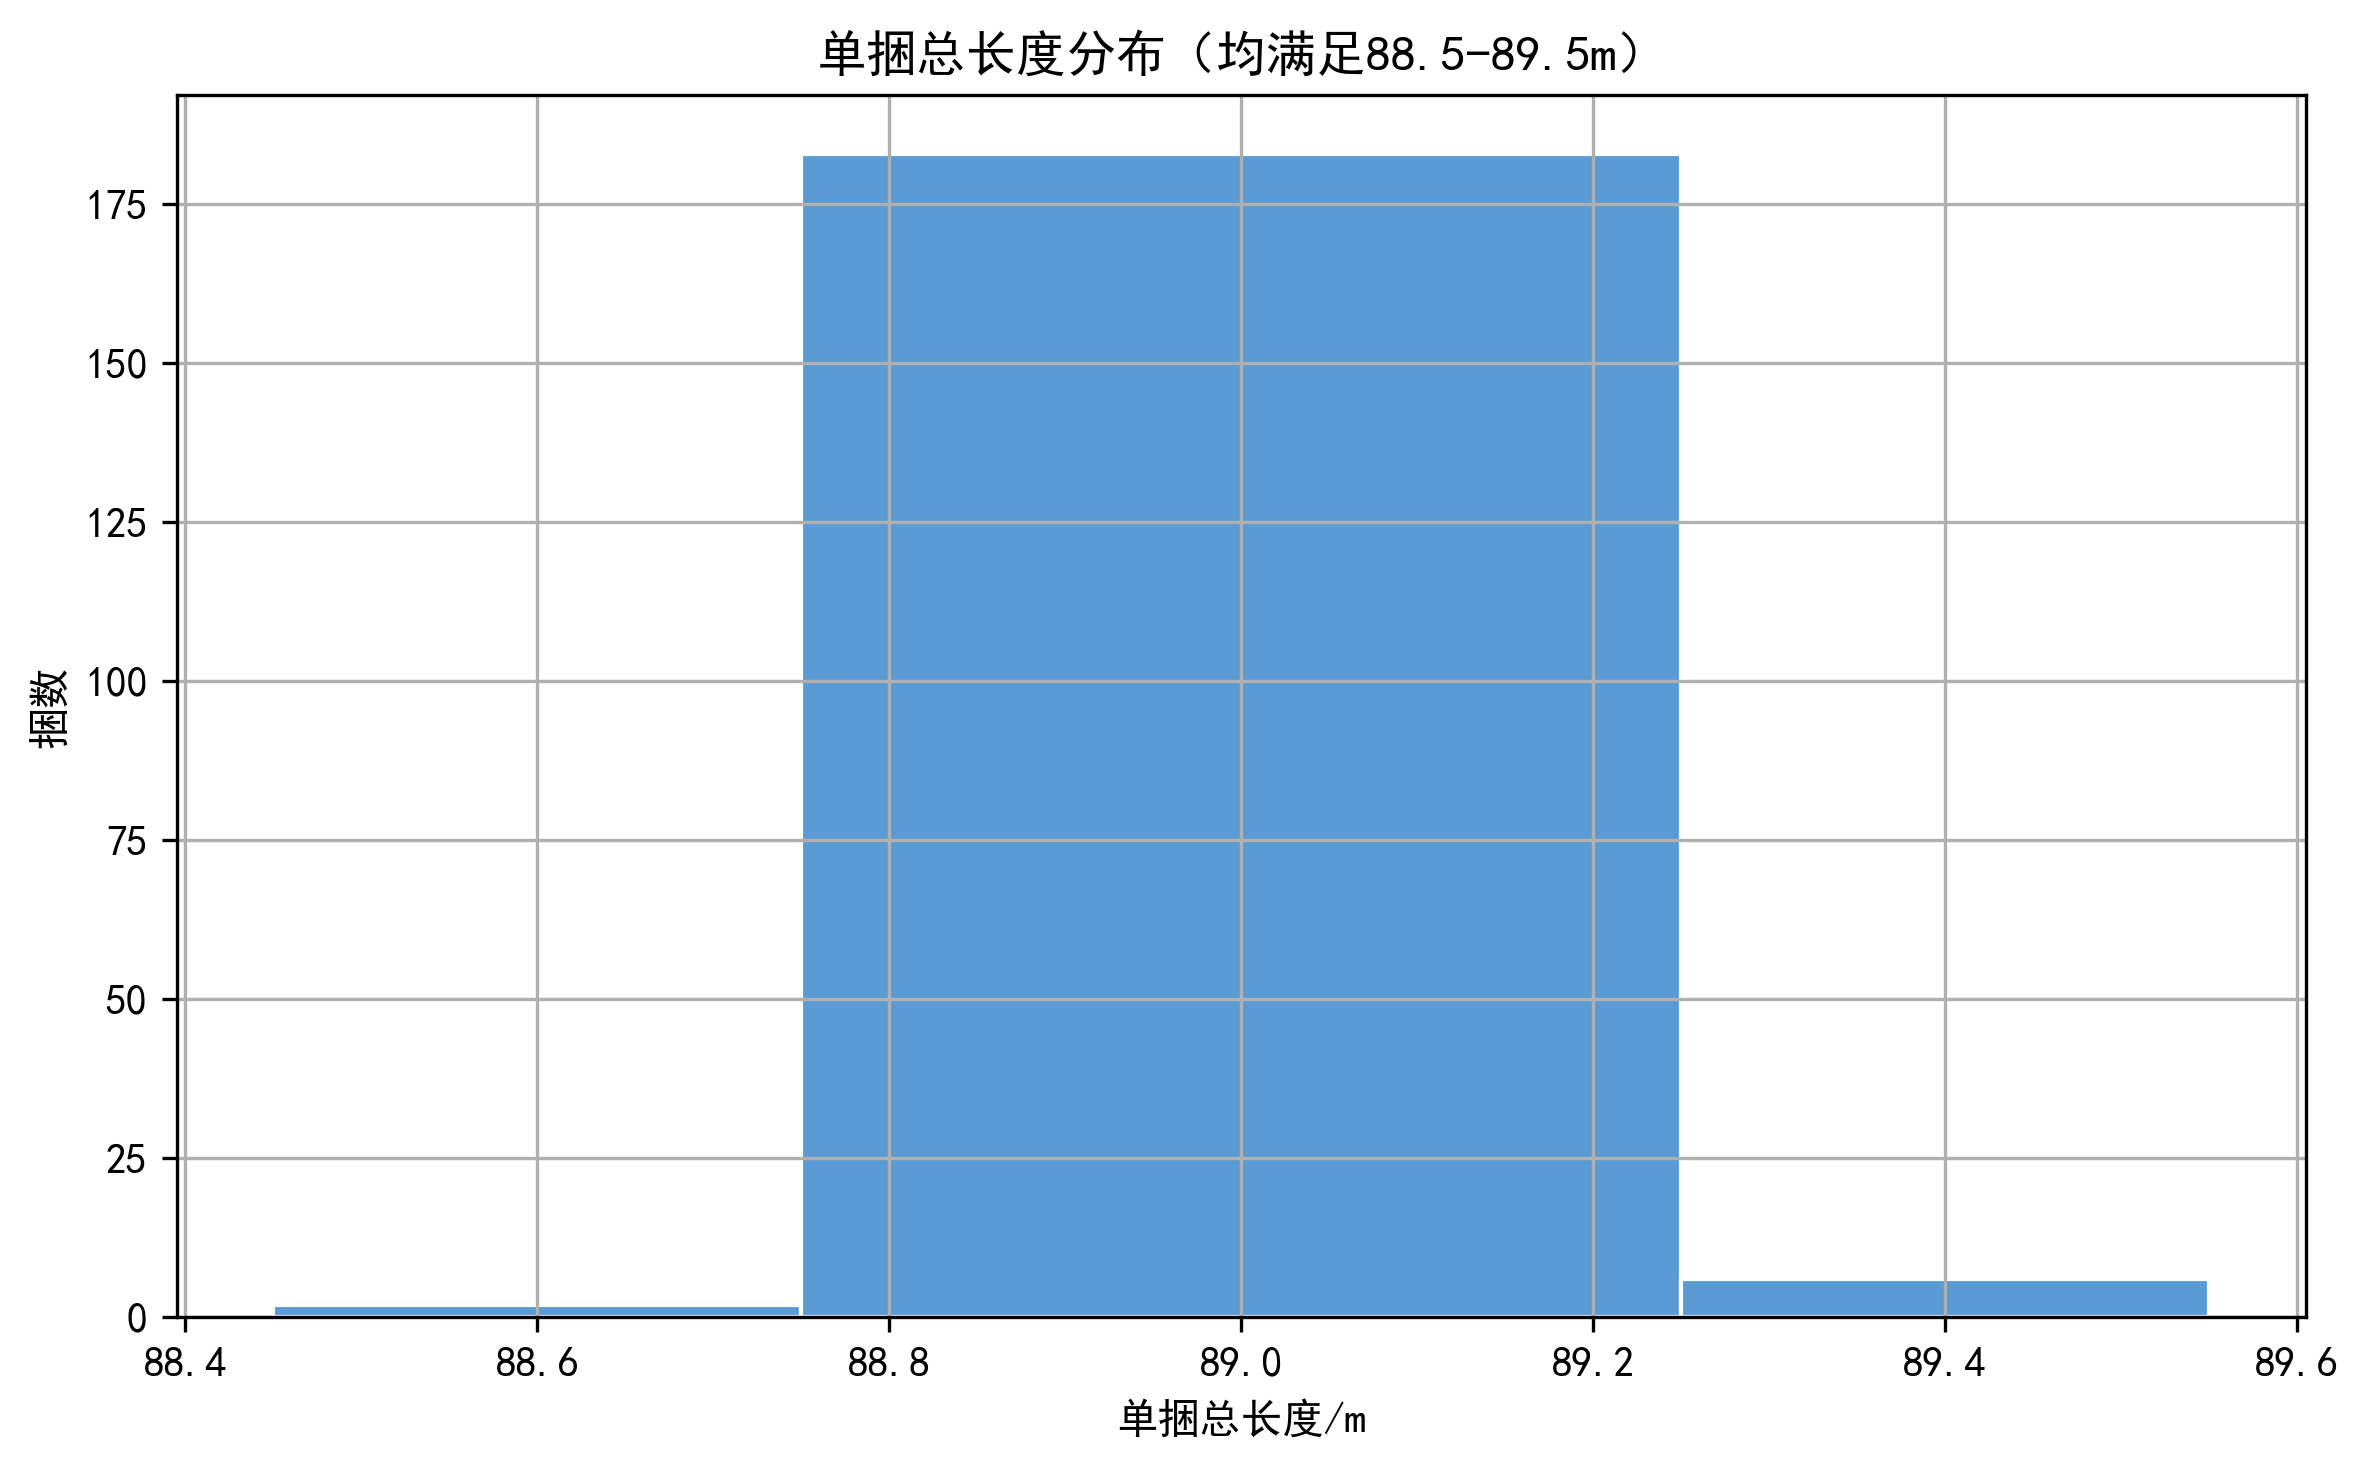
\includegraphics[width=0.75\textwidth]{../quest1/figures/fig4_bundle_length_distribution.png}
\caption{单捆总长度分布}
\label{fig:lengthdist}
\end{figure}

\section{模型评价与改进}
\subsection{模型优点}
第一，本文模型将“每捆合法性”前置到模式生成阶段，避免了聚合模型常见的伪可行问题。只要主问题选中的模式满足库存约束，展开后天然得到逐捆搭配清单，便于工人执行。

第二，字典序目标通过大权重分层实现，符合题目“先总捆数、再长规格、再中规格”的评价规则。相比单纯最大化长度利用率，该目标更贴近企业给定的方案优先级。

第三，稀疏模式池方法比直接为所有捆和所有长度档建立CP-SAT分配变量更容易获得高质量可行解，也比简单贪心更能利用全局库存信息。

\subsection{模型局限}
由于中规格和短规格合法模式数量巨大，本文采用受限模式池而非完整列生成，因此严格最优性未完全证明。191捆是已验证的高质量可行方案，而理论上界194捆和聚合上界并不能直接说明存在194捆逐捆方案。

此外，随机模式池的质量会影响最终结果。若增加模式生成轮数、引入列生成定价子问题或使用商业整数规划求解器，可能进一步搜索到192捆或更接近上界的方案。

\subsection{改进方向}
后续可将模式池方法扩展为列生成：主问题给出各长度档影子价格，定价问题按规格生成能改善目标的单捆模式，循环迭代直到没有改进列。这样既避免全模式枚举的内存爆炸，又能提供更强的最优性证据。

\section{结论}
本文针对天然肠衣搭配问题建立了合法单捆模式池与主整数规划模型，并对题目实际数据进行求解。最终得到的可执行方案为：共装出191捆，其中14米以上规格130捆、7--13.5米规格47捆、3--6.5米规格14捆。方案使用原料1302根、17001.0m，剩余21根、169.5m。独立验证表明，所有成品均满足单捆长度、根数、规格下限和库存约束，适合作为实际生产中的“照方抓药”搭配清单。

\section*{参考文献}
\addcontentsline{toc}{section}{参考文献}
\begin{enumerate}[label={[{\arabic*}]}]
  \item 全国大学生数学建模竞赛组委会. 2011高教社杯全国大学生数学建模竞赛D题：天然肠衣搭配问题[Z]. 2011.
  \item Gilmore P C, Gomory R E. A linear programming approach to the cutting-stock problem[J]. Operations Research, 1961, 9(6): 849--859.
  \item Martello S, Toth P. Knapsack Problems: Algorithms and Computer Implementations[M]. Wiley, 1990.
  \item Wolsey L A. Integer Programming[M]. Wiley, 1998.
  \item Achterberg T. Constraint Integer Programming[D]. Technische Universit\"at Berlin, 2007.
\end{enumerate}

\appendix
\section{支撑材料说明}
完整逐捆方案见\texttt{tables/final\_matching\_plan.csv}与\texttt{tables/final\_matching\_plan.xlsx}；各长度档库存使用情况见\texttt{tables/material\_usage\_by\_length.csv}；冻结数字见\texttt{results/frozen\_numbers.json}；验证报告见\texttt{results/validation\_report.json}。核心代码位于\texttt{quest1/codes/2011D\_sparse\_pattern\_pool.py}和\texttt{quest1/codes/validate\_final\_plan.py}。

\end{document}
